\documentclass{ximera}

\begin{document}

\begin{question}
  Find 
  \[
  \displaystyle \lim_{x\to-1} \frac{x^2+8x+7}{x^2+6x+5}
  \]
  \begin{solution}
    \begin{hint}
      This function is \underline{not} continuous everywhere, but both the numerator and denominator are continuous everywhere as functions. Thus, if the limit of $\frac{x^2+8x+7}{x^2+6x+5}$ as $x\to{a}$ does not exist, then the denominator $x^2+6x+5$ must be zero at $a$. Does $x^2+6x+5=0$ when $x=-1$? Does $x^2+8x+7=0$ at $x=-1$ as well?
    \end{hint}
     \begin{hint}
    Take a look at the graph of the function
    \begin{center}
     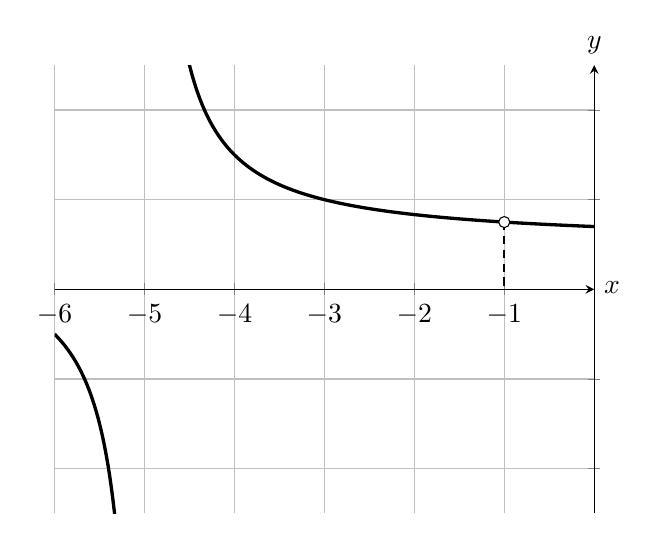
\begin{tikzpicture}
	\begin{axis}
	[ymin=-5,ymax=5, axis lines=center,xlabel=$x$,ylabel=$y$,every axis y 
	label/.style={at=(current axis.above origin),anchor=south},every axis x label/.style={at=(current axis.right of origin),anchor=west},
	domain=-6:0,
	yticklabels={},
	ymajorgrids=true,
	grid = major
	]
	\addplot[domain=-6:-501/100,very thick,smooth,samples=600]
	{(\x^2+8*\x+7)/(\x^2+6*\x+5)};
	\addplot[domain=-499/100:0,very thick,smooth,samples=600]
	{(\x^2+8*\x+7)/(\x^2+6*\x+5)};
	\draw[densely dashed, thick] (axis cs:-1,1.5)--(axis cs:-1,0);
	\draw[fill=white] (axis cs:-1,1.5) circle [radius=2pt];
	\end{axis}
       \end{tikzpicture}      
      \end{center}
      There is a removable discontinuity at $x=-1$. This suggests something about the factorization of both polynomials $x^2+8x+7$ and $x^2+6x+5$.
    \end{hint}
    \begin{hint}
     Notice that the quadratic equation tells us that $x^2+8x+7=0$ has solutions $-4\pm3$ and $x^2+6x+5=0$ has solutions $-3\pm{2}$. Thus, $x^2+8x+7=\left(x+1\right)\left(x+7\right)$ and $x^2+6x+5=\left(x+1\right)\left(x+5\right)$. Then $\lim\limits_{x\to-1}\frac{x^2+8x+7}{x^2+6x+5}=\lim\limits_{x\to-1}\frac{x+7}{x+5}$. 
    \end{hint}
    The limit, $\lim\limits_{x\to-1}\frac{x^2+8x+7}{x^2+5x+6}=$
    \answer{1.5}.
  \end{solution}
\end{question}

\end{document}